% Options for packages loaded elsewhere
\PassOptionsToPackage{unicode}{hyperref}
\PassOptionsToPackage{hyphens}{url}
%
\documentclass[
]{book}
\usepackage{amsmath,amssymb}
\usepackage{iftex}
\ifPDFTeX
  \usepackage[T1]{fontenc}
  \usepackage[utf8]{inputenc}
  \usepackage{textcomp} % provide euro and other symbols
\else % if luatex or xetex
  \usepackage{unicode-math} % this also loads fontspec
  \defaultfontfeatures{Scale=MatchLowercase}
  \defaultfontfeatures[\rmfamily]{Ligatures=TeX,Scale=1}
\fi
\usepackage{lmodern}
\ifPDFTeX\else
  % xetex/luatex font selection
\fi
% Use upquote if available, for straight quotes in verbatim environments
\IfFileExists{upquote.sty}{\usepackage{upquote}}{}
\IfFileExists{microtype.sty}{% use microtype if available
  \usepackage[]{microtype}
  \UseMicrotypeSet[protrusion]{basicmath} % disable protrusion for tt fonts
}{}
\makeatletter
\@ifundefined{KOMAClassName}{% if non-KOMA class
  \IfFileExists{parskip.sty}{%
    \usepackage{parskip}
  }{% else
    \setlength{\parindent}{0pt}
    \setlength{\parskip}{6pt plus 2pt minus 1pt}}
}{% if KOMA class
  \KOMAoptions{parskip=half}}
\makeatother
\usepackage{xcolor}
\usepackage{color}
\usepackage{fancyvrb}
\newcommand{\VerbBar}{|}
\newcommand{\VERB}{\Verb[commandchars=\\\{\}]}
\DefineVerbatimEnvironment{Highlighting}{Verbatim}{commandchars=\\\{\}}
% Add ',fontsize=\small' for more characters per line
\usepackage{framed}
\definecolor{shadecolor}{RGB}{248,248,248}
\newenvironment{Shaded}{\begin{snugshade}}{\end{snugshade}}
\newcommand{\AlertTok}[1]{\textcolor[rgb]{0.94,0.16,0.16}{#1}}
\newcommand{\AnnotationTok}[1]{\textcolor[rgb]{0.56,0.35,0.01}{\textbf{\textit{#1}}}}
\newcommand{\AttributeTok}[1]{\textcolor[rgb]{0.13,0.29,0.53}{#1}}
\newcommand{\BaseNTok}[1]{\textcolor[rgb]{0.00,0.00,0.81}{#1}}
\newcommand{\BuiltInTok}[1]{#1}
\newcommand{\CharTok}[1]{\textcolor[rgb]{0.31,0.60,0.02}{#1}}
\newcommand{\CommentTok}[1]{\textcolor[rgb]{0.56,0.35,0.01}{\textit{#1}}}
\newcommand{\CommentVarTok}[1]{\textcolor[rgb]{0.56,0.35,0.01}{\textbf{\textit{#1}}}}
\newcommand{\ConstantTok}[1]{\textcolor[rgb]{0.56,0.35,0.01}{#1}}
\newcommand{\ControlFlowTok}[1]{\textcolor[rgb]{0.13,0.29,0.53}{\textbf{#1}}}
\newcommand{\DataTypeTok}[1]{\textcolor[rgb]{0.13,0.29,0.53}{#1}}
\newcommand{\DecValTok}[1]{\textcolor[rgb]{0.00,0.00,0.81}{#1}}
\newcommand{\DocumentationTok}[1]{\textcolor[rgb]{0.56,0.35,0.01}{\textbf{\textit{#1}}}}
\newcommand{\ErrorTok}[1]{\textcolor[rgb]{0.64,0.00,0.00}{\textbf{#1}}}
\newcommand{\ExtensionTok}[1]{#1}
\newcommand{\FloatTok}[1]{\textcolor[rgb]{0.00,0.00,0.81}{#1}}
\newcommand{\FunctionTok}[1]{\textcolor[rgb]{0.13,0.29,0.53}{\textbf{#1}}}
\newcommand{\ImportTok}[1]{#1}
\newcommand{\InformationTok}[1]{\textcolor[rgb]{0.56,0.35,0.01}{\textbf{\textit{#1}}}}
\newcommand{\KeywordTok}[1]{\textcolor[rgb]{0.13,0.29,0.53}{\textbf{#1}}}
\newcommand{\NormalTok}[1]{#1}
\newcommand{\OperatorTok}[1]{\textcolor[rgb]{0.81,0.36,0.00}{\textbf{#1}}}
\newcommand{\OtherTok}[1]{\textcolor[rgb]{0.56,0.35,0.01}{#1}}
\newcommand{\PreprocessorTok}[1]{\textcolor[rgb]{0.56,0.35,0.01}{\textit{#1}}}
\newcommand{\RegionMarkerTok}[1]{#1}
\newcommand{\SpecialCharTok}[1]{\textcolor[rgb]{0.81,0.36,0.00}{\textbf{#1}}}
\newcommand{\SpecialStringTok}[1]{\textcolor[rgb]{0.31,0.60,0.02}{#1}}
\newcommand{\StringTok}[1]{\textcolor[rgb]{0.31,0.60,0.02}{#1}}
\newcommand{\VariableTok}[1]{\textcolor[rgb]{0.00,0.00,0.00}{#1}}
\newcommand{\VerbatimStringTok}[1]{\textcolor[rgb]{0.31,0.60,0.02}{#1}}
\newcommand{\WarningTok}[1]{\textcolor[rgb]{0.56,0.35,0.01}{\textbf{\textit{#1}}}}
\usepackage{longtable,booktabs,array}
\usepackage{calc} % for calculating minipage widths
% Correct order of tables after \paragraph or \subparagraph
\usepackage{etoolbox}
\makeatletter
\patchcmd\longtable{\par}{\if@noskipsec\mbox{}\fi\par}{}{}
\makeatother
% Allow footnotes in longtable head/foot
\IfFileExists{footnotehyper.sty}{\usepackage{footnotehyper}}{\usepackage{footnote}}
\makesavenoteenv{longtable}
\usepackage{graphicx}
\makeatletter
\def\maxwidth{\ifdim\Gin@nat@width>\linewidth\linewidth\else\Gin@nat@width\fi}
\def\maxheight{\ifdim\Gin@nat@height>\textheight\textheight\else\Gin@nat@height\fi}
\makeatother
% Scale images if necessary, so that they will not overflow the page
% margins by default, and it is still possible to overwrite the defaults
% using explicit options in \includegraphics[width, height, ...]{}
\setkeys{Gin}{width=\maxwidth,height=\maxheight,keepaspectratio}
% Set default figure placement to htbp
\makeatletter
\def\fps@figure{htbp}
\makeatother
\setlength{\emergencystretch}{3em} % prevent overfull lines
\providecommand{\tightlist}{%
  \setlength{\itemsep}{0pt}\setlength{\parskip}{0pt}}
\setcounter{secnumdepth}{5}
\usepackage{booktabs}
\ifLuaTeX
  \usepackage{selnolig}  % disable illegal ligatures
\fi
\usepackage[]{natbib}
\bibliographystyle{plainnat}
\usepackage{bookmark}
\IfFileExists{xurl.sty}{\usepackage{xurl}}{} % add URL line breaks if available
\urlstyle{same}
\hypersetup{
  pdftitle={Pronóstico de Ventas de Café en Máquinas Expendedoras},
  pdfauthor={Luisa Angélica Isaza Sanabria - Juan Andrés Murillo Cadena - Carlos Fabián Villa Infante},
  hidelinks,
  pdfcreator={LaTeX via pandoc}}

\title{Pronóstico de Ventas de Café en Máquinas Expendedoras}
\author{Luisa Angélica Isaza Sanabria - Juan Andrés Murillo Cadena - Carlos Fabián Villa Infante}
\date{2025-04-26}

\begin{document}
\maketitle

{
\setcounter{tocdepth}{1}
\tableofcontents
}
\chapter{Introducción}\label{introducciuxf3n}

Durante este curso de series de tiempo, hemos decidido trabajar las ventas de café en una máquina expendedora. Detrás de cada café que alguien compra, hay patrones de consumo, hábitos y decisiones que se repiten en el tiempo. Analizar esta información nos permite aplicar modelos de pronóstico reales, útiles y con impacto directo en la toma de decisiones comerciales y operativas.

Poder anticipar cuánto café se va a vender en los próximos días, semanas o meses es clave para mejorar la experiencia del cliente, reducir pérdidas y aumentar la eficiencia.

\section{Justificación de la Elección}\label{justificaciuxf3n-de-la-elecciuxf3n}

El café es una de las bebidas más consumidas en todo el mundo, y las máquinas expendedoras son una forma práctica de acceder a él. Nos pareció un caso ideal porque:

\begin{verbatim}
1.  Ayuda a planificar mejor los inventarios: Prever la demanda permite tener siempre lo justo: ni mucho producto que termine vencido, ni tan poco que dejemos de vender.

2.  Hace más eficientes las operaciones: Si sabemos cuándo se vende más café, podemos organizar mejor las recargas y los mantenimientos, ahorrando tiempo y dinero.

3.  Permite personalizar promociones:Detectar días u horarios de baja demanda ayuda a lanzar promociones en momentos estratégicos.

4.  Mejora la experiencia de quienes compran: Asegurar que los productos favoritos estén disponibles en los momentos clave mejora la satisfacción y fideliza al cliente.
\end{verbatim}

\section{Descripción de la Información a Utilizar}\label{descripciuxf3n-de-la-informaciuxf3n-a-utilizar}

Vamos a utilizar un dataset llamado ``Coffee Sales'', publicado por Yaroslav Isaienkov en la plataforma Kaggle. Esta base de datos contiene registros reales de ventas desde marzo de 2024 y sigue actualizándose semanalmente.

El dataset incluye:

\begin{verbatim}
•   La fecha y hora de cada transacción
•   El tipo de café vendido
•   La cantidad y el método de pago
•   Información detallada sobre el producto y las preferencias del cliente
\end{verbatim}

Todo esto en archivos están en formato .csv que son muy fáciles de trabajar y analizar, ideales para aplicar modelos de series de tiempo.

\section{Fuentes y Permisos de Uso}\label{fuentes-y-permisos-de-uso}

Una gran ventaja de este dataset es que está disponible bajo una licencia de dominio público (CC0),(\citet{isaienkov2025}) lo que significa que se puede usar libremente con fines educativos, de análisis y sin restricciones. Además, todos los datos han sido recolectados de forma anónima a partir de informes de la propia máquina expendedora.

\chapter{Análisis grafico de series de tiempo}\label{anuxe1lisis-grafico-de-series-de-tiempo}

Este es un análisis temporal de las ventas diarias de una máquina de café, con el objetivo de identificar patrones, tendencias y ciclos estacionales que permitan optimizar la gestión del negocio. Los datos incluyen información sobre la fecha y hora de las ventas, el medio de pago (efectivo o tarjeta), el valor de cada transacción y el tipo de café vendido. El análisis se centra en la variable \texttt{valor\_total} (suma de ventas por día) y utiliza tres herramientas principales: el promedio móvil, la función de autocorrelación (ACF) y la descomposición STL.

\section{Metodología}\label{metodologuxeda}

\subsection{Datos}\label{datos}

Los datos abarcan un periodo de 385 días, desde abril 01 de 2024 hasta abril 23 de 2025. La variable analizada, \texttt{valor\_total}, representa la suma de las ventas diarias (en dolares).

\subsection{Promedio móvil}\label{promedio-muxf3vil}

Promedio móvil: Se calculó un promedio móvil de 7 días para suavizar las fluctuaciones diarias y destacar tendencias generales en las ventas. La siguiente gráfica muestra las ventas diarias (línea azul) junto con el promedio móvil (línea naranja).

\begin{figure}
\centering
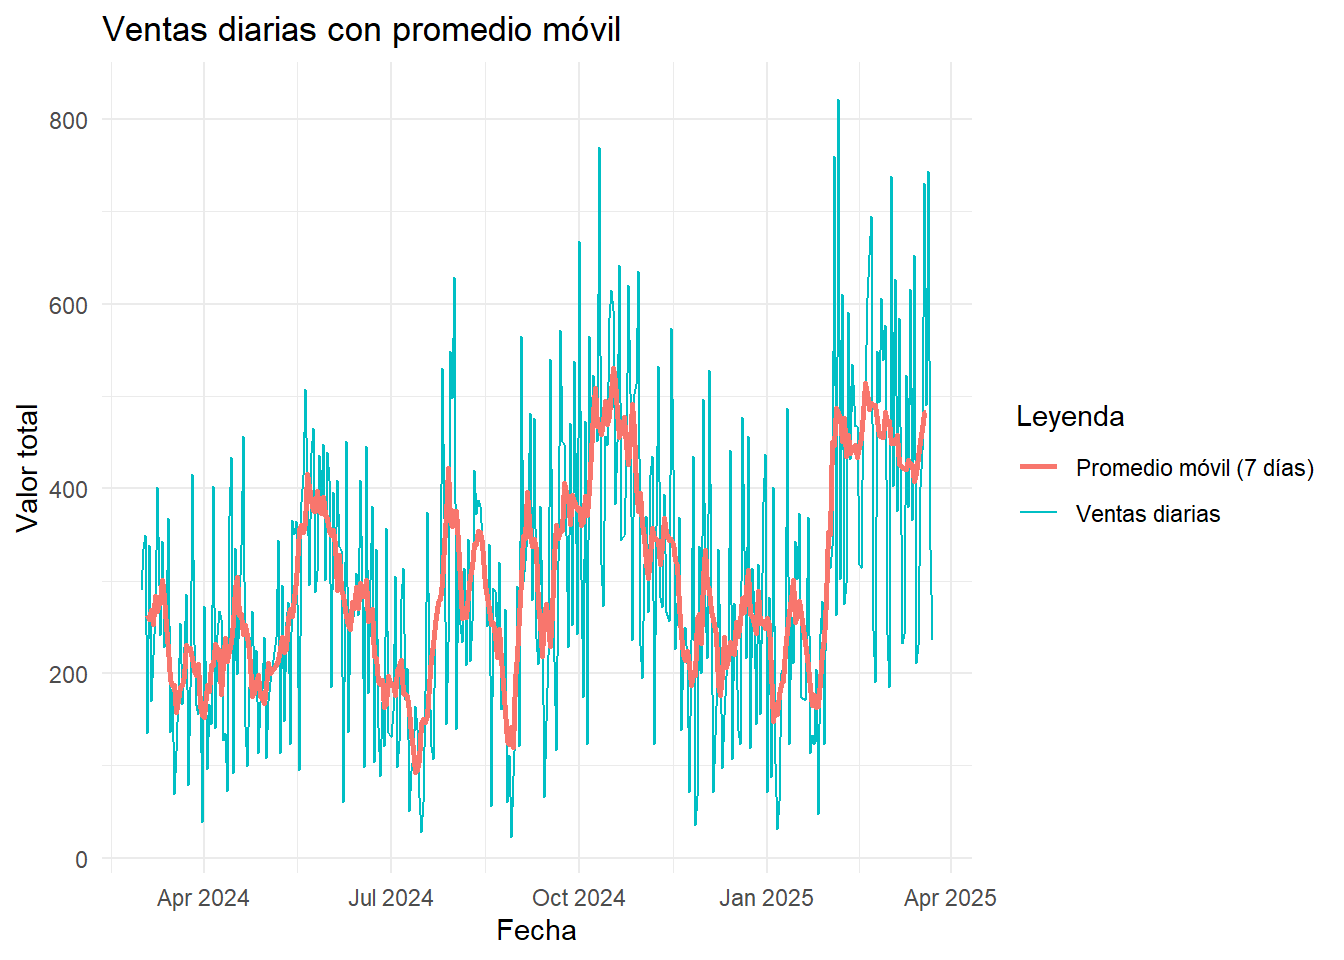
\includegraphics{_main_files/figure-latex/promedio-movil-1.pdf}
\caption{\label{fig:promedio-movil}Ventas diarias con promedio móvil}
\end{figure}

La gráfica muestra una alta variabilidad en las ventas diarias, con picos que alcanzan hasta 800 y caídas cercanas a 0. El promedio móvil revela las siguientes tendencias:
Abril-julio 2024: Las ventas promedio crecen de \textasciitilde300 a \textasciitilde400, indicando un aumento en la demanda.

Julio-octubre 2024: Alcanzan un pico de \textasciitilde500, mostrando un periodo de alta demanda, posiblemente por festividades o factores estacionales.

Octubre 2024-enero 2025: Disminuyen a \textasciitilde300, reflejando una caída en las ventas durante el invierno.

Enero-abril 2025: Se recuperan y estabilizan en \textasciitilde400, indicando una mejora en la primavera.

Esto sugiere una tendencia estacional a largo plazo, con un pico en octubre y una caída en invierno.

\subsection{Función de Autocorrelación (ACF)}\label{funciuxf3n-de-autocorrelaciuxf3n-acf}

La función de autocorrelación (ACF) mide la correlación de las ventas diarias consigo mismas en diferentes rezagos, ayudando a identificar patrones temporales y ciclos estacionales.

\begin{Shaded}
\begin{Highlighting}[]
\CommentTok{\# Función para calcular rezagos}
\NormalTok{calcular\_rezagos }\OtherTok{\textless{}{-}} \ControlFlowTok{function}\NormalTok{(serie, }\AttributeTok{lag\_max =} \DecValTok{14}\NormalTok{) \{}
  \FunctionTok{acf}\NormalTok{(serie, }\AttributeTok{lag.max =}\NormalTok{ lag\_max, }\AttributeTok{plot =} \ConstantTok{FALSE}\NormalTok{)}
\NormalTok{\}}

\CommentTok{\# Calcular autocorrelación}

\NormalTok{acf\_ventas }\OtherTok{\textless{}{-}} \FunctionTok{calcular\_rezagos}\NormalTok{(ts\_ventas)}
\FunctionTok{autoplot}\NormalTok{(acf\_ventas) }\SpecialCharTok{+}
  \FunctionTok{labs}\NormalTok{(}\AttributeTok{title =} \StringTok{"Función de autocorrelación (ACF) de ventas diarias"}\NormalTok{,}
       \AttributeTok{x =} \StringTok{"Rezago (días)"}\NormalTok{, }\AttributeTok{y =} \StringTok{"Autocorrelación"}\NormalTok{) }\SpecialCharTok{+}
  \FunctionTok{theme\_minimal}\NormalTok{()}
\end{Highlighting}
\end{Shaded}

\begin{figure}
\centering
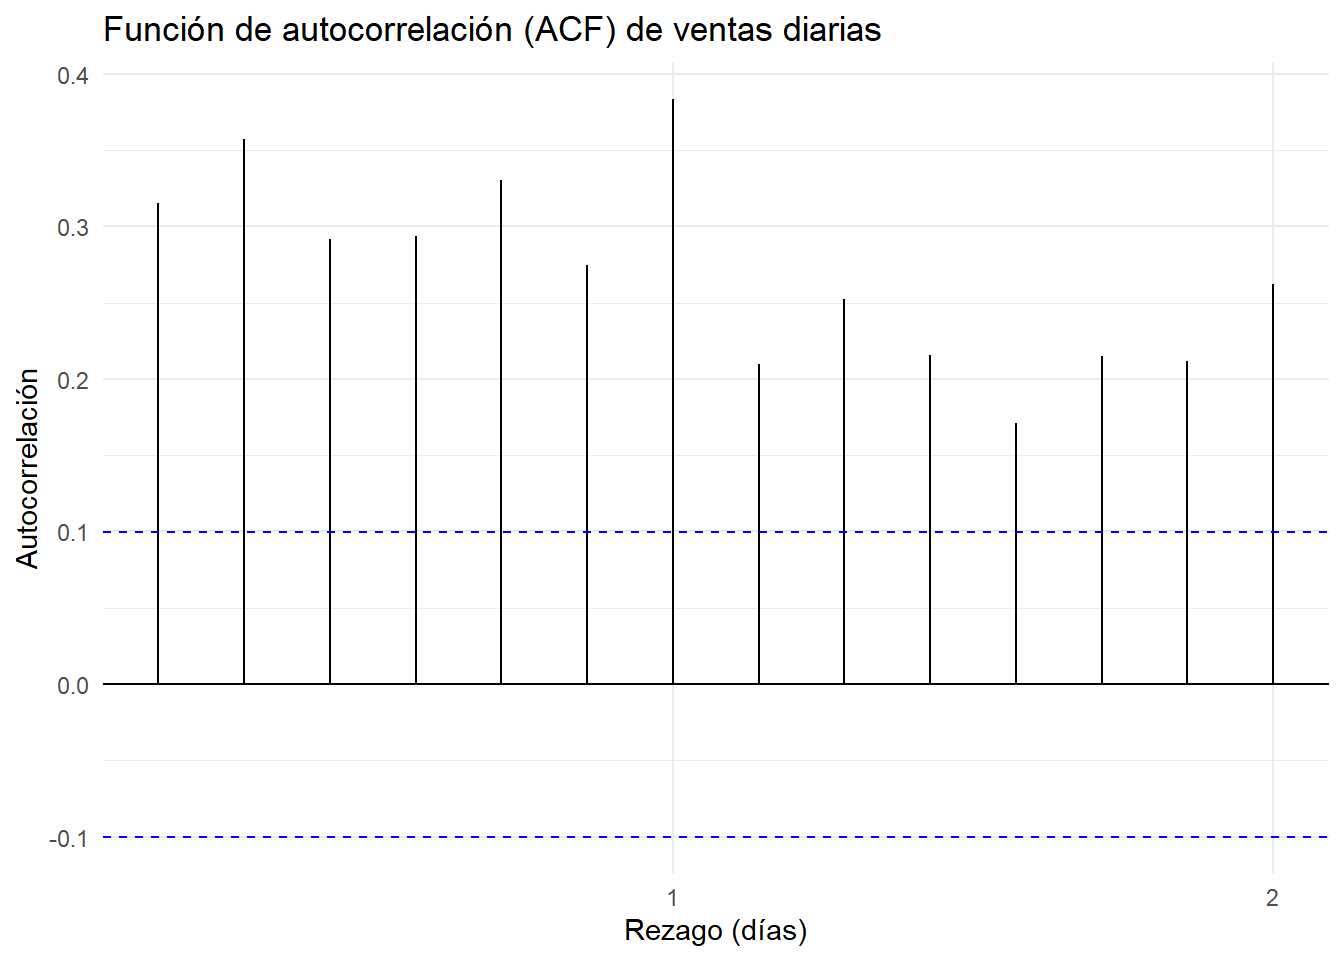
\includegraphics{_main_files/figure-latex/rezagos-1.pdf}
\caption{\label{fig:rezagos}Autocorrelación de ventas}
\end{figure}

La gráfica ACF muestra:
Rezagos 1 a 6: Autocorrelaciones significativas (\textasciitilde0.3 a 0.4), indicando una dependencia a corto plazo. Las ventas de un día están correlacionadas con las de los días anteriores, con un efecto que disminuye gradualmente.

Rezago 7: Un pico significativo (\textasciitilde0.4), confirmando un ciclo semanal. Esto indica que las ventas tienen un patrón que se repite cada 7 días (por ejemplo, mayor demanda los fines de semana).

Rezagos 8 a 14: Autocorrelaciones más pequeñas pero aún significativas, con otro pico en el rezago 14 (segundo ciclo semanal), reforzando el patrón estacional.

Este ciclo semanal sugiere que las ventas varían según el día de la semana.

\subsection{Descomposición STL}\label{descomposiciuxf3n-stl}

La descomposición STL separa la serie temporal en tres componentes: tendencia, estacionalidad (ciclo semanal) y residuo.

\begin{Shaded}
\begin{Highlighting}[]
\CommentTok{\# Verifica la serie temporal}
\FunctionTok{print}\NormalTok{(ts\_ventas)}
\end{Highlighting}
\end{Shaded}

\begin{verbatim}
## Time Series:
## Start = c(1, 1) 
## End = c(55, 7) 
## Frequency = 7 
##   [1] 290.00 334.40 349.10 135.20 338.50 170.20 220.10 265.50 402.00 241.40
##  [11] 342.80 228.10 256.20 368.20 136.50 183.20  68.90 115.60 179.90 253.90
##  [21] 166.50 228.10 285.10  78.70 184.90 415.40 231.70 165.40 156.10 189.90
##  [31]  38.70 272.80  96.50 166.50 145.00 402.10 140.10 241.50 267.70 258.60
##  [41] 127.70 135.20  72.50 370.00 434.30  91.60 335.30 199.20 275.30 338.50
##  [51] 456.58 142.36  99.74 184.98 267.46 192.02 224.84 113.16 169.00 182.22
##  [61] 239.54 108.26 170.28 189.88 239.14 344.08 113.16 295.38 148.44 255.52
##  [71] 277.26 123.64 365.92 350.82 365.06  94.74 385.52 414.22 508.08 403.56
##  [81] 295.38 437.94 465.66 287.74 310.08 436.46 391.70 447.54 300.28 439.22
##  [91] 408.54 184.98 396.50 307.54 408.54 338.00 333.10  60.74 451.16 136.18
## [101] 259.14 254.24 267.46 308.60 262.56 408.54 290.48  98.46 446.26 178.80
## [111] 300.28 380.62 103.36 334.58 141.08  88.66 169.00 121.48 357.60 136.18
## [121] 131.28 159.20 305.18  98.46 126.38 280.68 313.50 172.42 205.24  50.94
## [131]  93.56 111.68 164.10 139.60  65.64  27.92  60.74 180.74 374.24 200.34
## [141] 121.48 106.78 261.08 269.40 279.20 530.48 367.86 144.50 233.16 548.60
## [151] 497.66 628.94 139.60 325.24 252.76 233.16 313.50 208.66 344.84 213.56
## [161] 256.18 420.28 372.76 387.46 381.08 344.84 310.54 251.28 339.94  55.84
## [171] 292.42 289.00 233.16 320.34 161.14 167.52 269.40  60.74 111.68  23.02
## [181]  88.66 143.02 293.90 121.48 564.78 298.80 321.82 353.16 481.48 279.20
## [191] 476.12 238.06 210.14 381.08 265.98  65.64 147.92 219.94 540.28 303.70
## [201] 213.56 116.58 321.82 571.62 451.62 448.20 349.74 228.26 471.22 251.78
## [211] 537.86 241.98 667.66 302.24 173.90 472.70 123.44 565.28 435.48 523.16
## [221] 498.66 451.64 770.04 318.40 272.84 456.54 446.74 584.88 614.28 593.22
## [231] 383.56 450.18 641.70 344.36 349.26 430.58 620.64 503.56 235.62 502.10
## [241] 513.36 635.34 230.72 194.96 318.40 370.32 266.48 414.42 435.48 123.44
## [251] 359.06 532.96 282.64 271.38 393.36 266.48 256.68 573.62 420.78 225.82
## [261] 276.28 368.86 138.14 225.82 250.32 211.12  71.52 235.62 435.48  35.76
## [271]  66.62 338.00 199.86 497.20 272.84 216.02 528.06 282.64  71.52 164.10
## [281] 334.56 216.02  97.48 154.30 196.42 230.72 441.84 107.28 276.28 225.82
## [291] 138.14 123.44 477.60 333.10 216.02 456.54 118.54 313.50 266.48 144.50
## [301] 318.40 155.76 385.02 436.94  71.52 282.64  87.68 401.18 102.38  30.86
## [311]  61.72 199.86 206.22 230.72 487.40 123.44 261.58 211.12 342.90 302.24
## [321] 373.76 173.90 170.46 368.86 113.64 133.24 123.44 204.76  47.02 241.98
## [331] 277.74 123.44 324.76 333.10 313.50 338.00 760.24 263.04 821.96 302.24
## [341] 610.84 274.30 297.34 591.24 432.04 534.42 467.80 467.80 318.40 313.50
## [351] 505.02 505.02 605.94 652.96 695.08 246.88 190.06 549.12 493.76 605.94
## [361] 539.32 576.54 241.98 185.16 737.72 402.64 627.00 375.22 584.88 232.18
## [371] 241.98 523.16 380.12 615.74 365.42 652.96 211.12 230.72 401.18 441.84
## [381] 730.84 490.32 744.08 334.56 235.62
\end{verbatim}

\begin{Shaded}
\begin{Highlighting}[]
\CommentTok{\# Asegúrate de que ts\_ventas tiene 391 días}
\FunctionTok{length}\NormalTok{(ts\_ventas)  }\CommentTok{\# Debería devolver 391}
\end{Highlighting}
\end{Shaded}

\begin{verbatim}
## [1] 385
\end{verbatim}

\begin{Shaded}
\begin{Highlighting}[]
\CommentTok{\# Aplica STL}
\NormalTok{descomposicion }\OtherTok{\textless{}{-}} \FunctionTok{stl}\NormalTok{(ts\_ventas, }\AttributeTok{s.window =} \StringTok{"periodic"}\NormalTok{)}

\CommentTok{\# Grafica}
\FunctionTok{autoplot}\NormalTok{(descomposicion) }\SpecialCharTok{+}
  \FunctionTok{labs}\NormalTok{(}\AttributeTok{title =} \StringTok{"Descomposición de la serie temporal de ventas"}\NormalTok{,}
       \AttributeTok{x =} \StringTok{"Días transcurridos"}\NormalTok{)}
\end{Highlighting}
\end{Shaded}

\begin{figure}
\centering
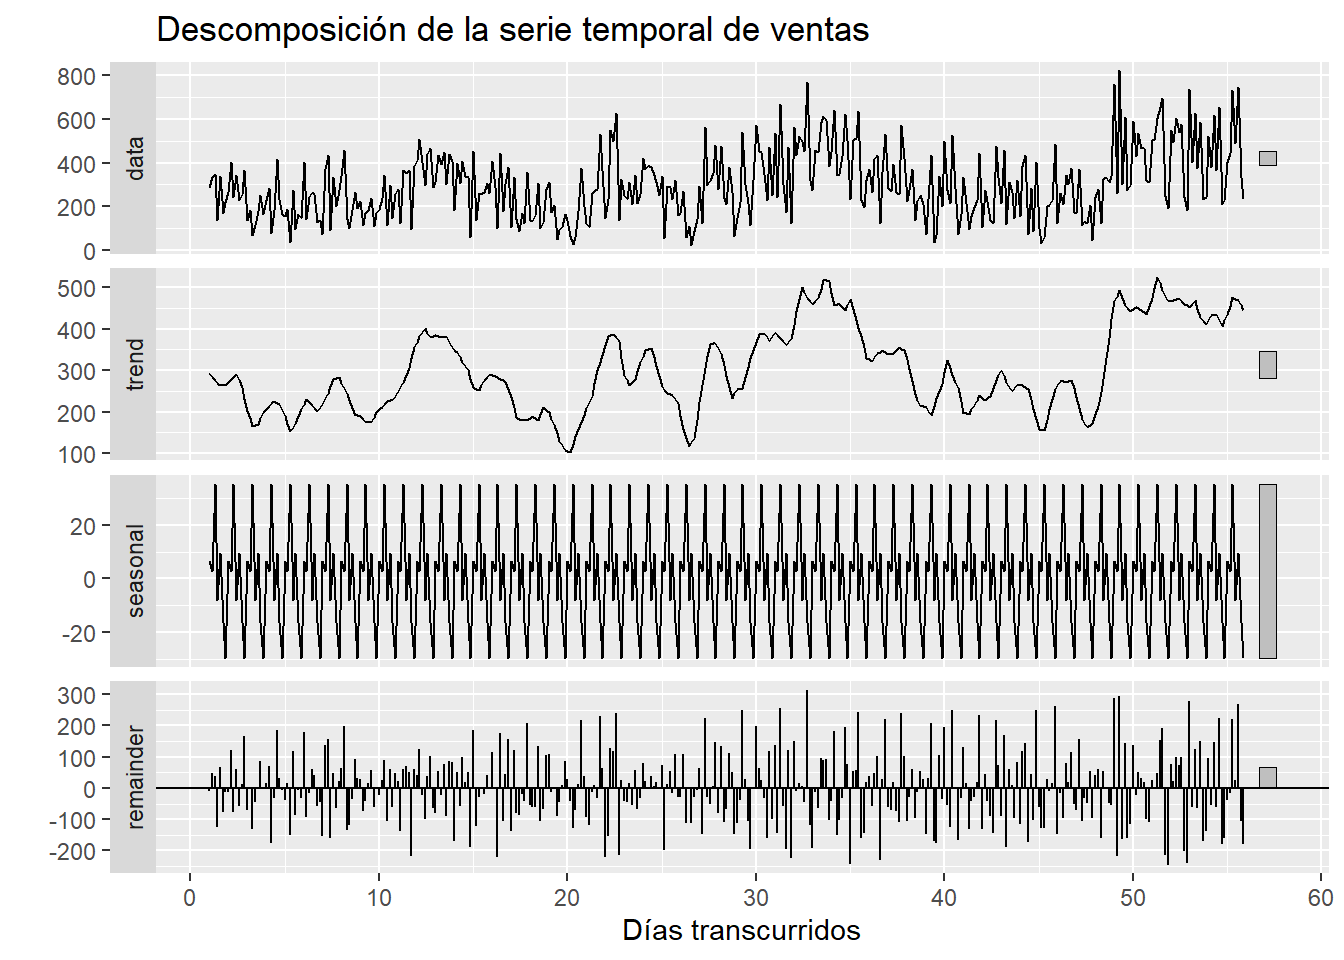
\includegraphics{_main_files/figure-latex/estacionalidad-1.pdf}
\caption{\label{fig:estacionalidad}Descomposición de la serie temporal}
\end{figure}

\begin{Shaded}
\begin{Highlighting}[]
\CommentTok{\# Extraer los componentes de la descomposición STL}
\NormalTok{stl\_components }\OtherTok{\textless{}{-}} \FunctionTok{as.data.frame}\NormalTok{(descomposicion}\SpecialCharTok{$}\NormalTok{time.series)}
\NormalTok{stl\_components}\SpecialCharTok{$}\NormalTok{fecha }\OtherTok{\textless{}{-}}\NormalTok{ ventas\_diarias}\SpecialCharTok{$}\NormalTok{fecha}

\CommentTok{\# Verificar que las fechas coincidan}
\FunctionTok{head}\NormalTok{(stl\_components}\SpecialCharTok{$}\NormalTok{fecha)}
\end{Highlighting}
\end{Shaded}

\begin{verbatim}
## [1] "2024-03-01" "2024-03-02" "2024-03-03" "2024-03-04" "2024-03-05"
## [6] "2024-03-06"
\end{verbatim}

\begin{Shaded}
\begin{Highlighting}[]
\FunctionTok{tail}\NormalTok{(stl\_components}\SpecialCharTok{$}\NormalTok{fecha)}
\end{Highlighting}
\end{Shaded}

\begin{verbatim}
## [1] "2025-03-18" "2025-03-19" "2025-03-20" "2025-03-21" "2025-03-22"
## [6] "2025-03-23"
\end{verbatim}

\begin{Shaded}
\begin{Highlighting}[]
\CommentTok{\# Crear una gráfica personalizada con ggplot2}
\FunctionTok{library}\NormalTok{(ggplot2)}

\CommentTok{\# Gráfica de todos los componentes}
\NormalTok{p1 }\OtherTok{\textless{}{-}} \FunctionTok{ggplot}\NormalTok{(stl\_components, }\FunctionTok{aes}\NormalTok{(}\AttributeTok{x =}\NormalTok{ fecha)) }\SpecialCharTok{+}
  \FunctionTok{geom\_line}\NormalTok{(}\FunctionTok{aes}\NormalTok{(}\AttributeTok{y =}\NormalTok{ seasonal }\SpecialCharTok{+}\NormalTok{ trend }\SpecialCharTok{+}\NormalTok{ remainder, }\AttributeTok{color =} \StringTok{"Datos"}\NormalTok{)) }\SpecialCharTok{+}
  \FunctionTok{labs}\NormalTok{(}\AttributeTok{title =} \StringTok{"Datos originales"}\NormalTok{, }\AttributeTok{y =} \StringTok{"Ventas"}\NormalTok{) }\SpecialCharTok{+}
  \FunctionTok{theme\_minimal}\NormalTok{()}

\NormalTok{p2 }\OtherTok{\textless{}{-}} \FunctionTok{ggplot}\NormalTok{(stl\_components, }\FunctionTok{aes}\NormalTok{(}\AttributeTok{x =}\NormalTok{ fecha)) }\SpecialCharTok{+}
  \FunctionTok{geom\_line}\NormalTok{(}\FunctionTok{aes}\NormalTok{(}\AttributeTok{y =}\NormalTok{ trend, }\AttributeTok{color =} \StringTok{"Tendencia"}\NormalTok{)) }\SpecialCharTok{+}
  \FunctionTok{labs}\NormalTok{(}\AttributeTok{title =} \StringTok{"Tendencia"}\NormalTok{, }\AttributeTok{y =} \StringTok{"Ventas"}\NormalTok{) }\SpecialCharTok{+}
  \FunctionTok{theme\_minimal}\NormalTok{()}

\NormalTok{p3 }\OtherTok{\textless{}{-}} \FunctionTok{ggplot}\NormalTok{(stl\_components, }\FunctionTok{aes}\NormalTok{(}\AttributeTok{x =}\NormalTok{ fecha)) }\SpecialCharTok{+}
  \FunctionTok{geom\_line}\NormalTok{(}\FunctionTok{aes}\NormalTok{(}\AttributeTok{y =}\NormalTok{ seasonal, }\AttributeTok{color =} \StringTok{"Estacionalidad"}\NormalTok{)) }\SpecialCharTok{+}
  \FunctionTok{labs}\NormalTok{(}\AttributeTok{title =} \StringTok{"Estacionalidad"}\NormalTok{, }\AttributeTok{y =} \StringTok{"Ventas"}\NormalTok{) }\SpecialCharTok{+}
  \FunctionTok{theme\_minimal}\NormalTok{()}

\NormalTok{p4 }\OtherTok{\textless{}{-}} \FunctionTok{ggplot}\NormalTok{(stl\_components, }\FunctionTok{aes}\NormalTok{(}\AttributeTok{x =}\NormalTok{ fecha)) }\SpecialCharTok{+}
  \FunctionTok{geom\_line}\NormalTok{(}\FunctionTok{aes}\NormalTok{(}\AttributeTok{y =}\NormalTok{ remainder, }\AttributeTok{color =} \StringTok{"Residuo"}\NormalTok{)) }\SpecialCharTok{+}
  \FunctionTok{labs}\NormalTok{(}\AttributeTok{title =} \StringTok{"Residuo"}\NormalTok{, }\AttributeTok{y =} \StringTok{"Ventas"}\NormalTok{) }\SpecialCharTok{+}
  \FunctionTok{theme\_minimal}\NormalTok{()}

\CommentTok{\# Combinar gráficos}
\FunctionTok{library}\NormalTok{(patchwork)}
\NormalTok{p1 }\SpecialCharTok{/}\NormalTok{ p2 }\SpecialCharTok{/}\NormalTok{ p3 }\SpecialCharTok{/}\NormalTok{ p4}
\end{Highlighting}
\end{Shaded}

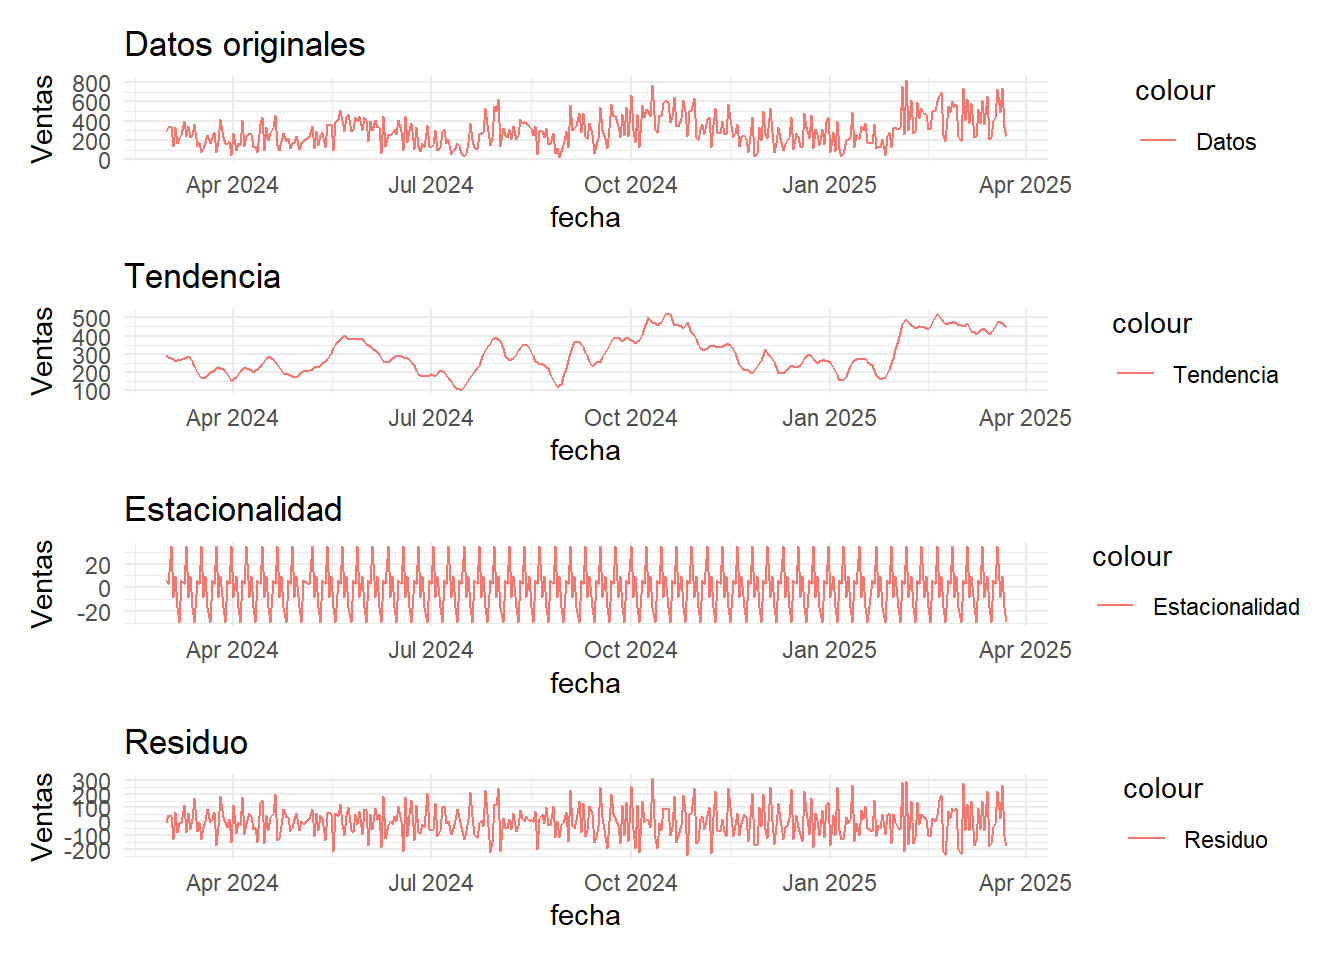
\includegraphics{_main_files/figure-latex/arreglo-1.pdf}

La descomposición STL revela los siguientes patrones:
Tendencia: Similar al promedio móvil, muestra un aumento inicial (abril-julio 2024), un pico en octubre (500), una caída en invierno (300), y una recuperación en primavera (\textasciitilde400). Esto confirma una tendencia estacional a largo plazo.

Estacionalidad: Oscila entre -20 y 20, con un ciclo que se repite cada 7 días, confirmando el patrón semanal identificado por la ACF. Aunque el efecto estacional es pequeño, indica variaciones según el día de la semana (por ejemplo, mayor demanda los fines de semana).

Residuo: Varía entre -300 y 300, mostrando una alta variabilidad. Esto indica que hay fluctuaciones significativas en las ventas que no se explican por la tendencia ni la estacionalidad, posiblemente debido a eventos aleatorios (festivos, promociones, cierres).

\section{Conclusiones}\label{conclusiones}

El análisis temporal de las ventas diarias de la máquina de café revela los siguientes hallazgos:
Tendencia estacional a largo plazo: Las ventas crecen hacia octubre (pico de 500), caen en invierno (300), y se recuperan en primavera (\textasciitilde400).

Ciclo semanal: Tanto la ACF como la descomposición STL confirman un ciclo de 7 días, indicando que las ventas varían según el día de la semana. Se puede analizar las ventas por día de la semana para identificar días de alta demanda (por ejemplo, fines de semana).

Alta variabilidad residual: El residuo de la descomposición STL muestra fluctuaciones significativas (hasta ±300), lo que sugiere que las ventas tienen un componente impredecible. Esto podría deberse a eventos externos (festivos, promociones), que vale la pena investigar para mejorar las predicciones.

En resumen, las ventas de la máquina de café presentan patrones claros a nivel semanal y estacional. Sin embargo, la alta variabilidad residual indica la necesidad de un análisis más profundo de factores externos para mejorar la previsión y gestión del negocio.

  \bibliography{book.bib,packages.bib}

\end{document}
